\section{Software System Definitions}

As in any large-scale system with multiple subsystems, the must be common system-level definitions that are obeyed by all subsystems. In the robot's software, too, there are common definitions obeyed by all layers of code in LabVIEW and in ROS. As such, this section will detail the common software system definitions.

\subsection{The Vehicle Co-Ordinate System}

The vehicle co-ordinate system is defined using the standard used on most ground vehicles: with the positive x direction straight ahead. In order to maintain a right-handed co-ordinate system, the three axes of the vehicle co-ordinate system are therefore defined as:

\begin{enumerate}
\item The positive X axis is pointed to the front of the vehicle
\item The positive Y axis is pointed to the left of the vehicle
\item The positive Z axis is pointed upward
\end{enumerate}

\begin{figure}[h!]
\centering

\includegraphics[scale=.7]{Photos/veh_coord.png}
\caption{Vehicle Co-ordinate System Definition}
\label{fig:veh_coord}
\end{figure} 


\newpage

\noindent The respective rotations in the vehicle co-ordinate system are therefore defined as:

\begin{enumerate}
\item Positive rotation about the X axis (Positive Roll) is roll toward the driver's right side of the vehicle
\item Positive rotation about the Y axis (Positive Pitch) is pitch downward toward the ground
\item Positive rotation about the Z axis (Positive Yaw) is yaw toward the driver's left side (counter clockwise yaw) of the vehicle
\end{enumerate}

\newpage

\subsection{LIDAR Co-Ordinate Definition}
By default, the Sick LMS290 LIDARs are programmed to transmit distance measurements in millimeters (mm) and angles in degrees with 0 degrees on the right and 180 degrees on the left as shown in the image below:

\begin{figure}[h!]
\centering
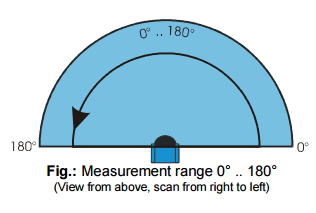
\includegraphics[scale=.9]{Photos/LIDAR_AngleDef.png}
\caption[Sick LMS290 Angle Definition]{Sick LMS290 Angle Definition \protect \footnotemark}
\label{fig:sick_angledef}
\end{figure} 
\footnotetext{ Information obtained from Quick Manual for LMS Communication Setup}